\documentclass[12pt, letterpaper]{article}
\usepackage{graphicx}

\title{\LaTeX \ 30}
\author{Gordon Chen\thanks{Created by Parents}}
\date{Fall 2026}

\begin{document}
\maketitle  % this is a comment.

\begin{abstract}
    This is \LaTeX.
\end{abstract}

\tableofcontents

\section{Text}
I can write in \textbf{bold} and \textit{italics}.
I can also \underline{underline}.

I can \emph{emphasize}, \textbf{emphasize \emph{again}}, and \textit{emphasize \emph{again}}.


\section{Image}
\begin{figure}[ht]
    \centering
    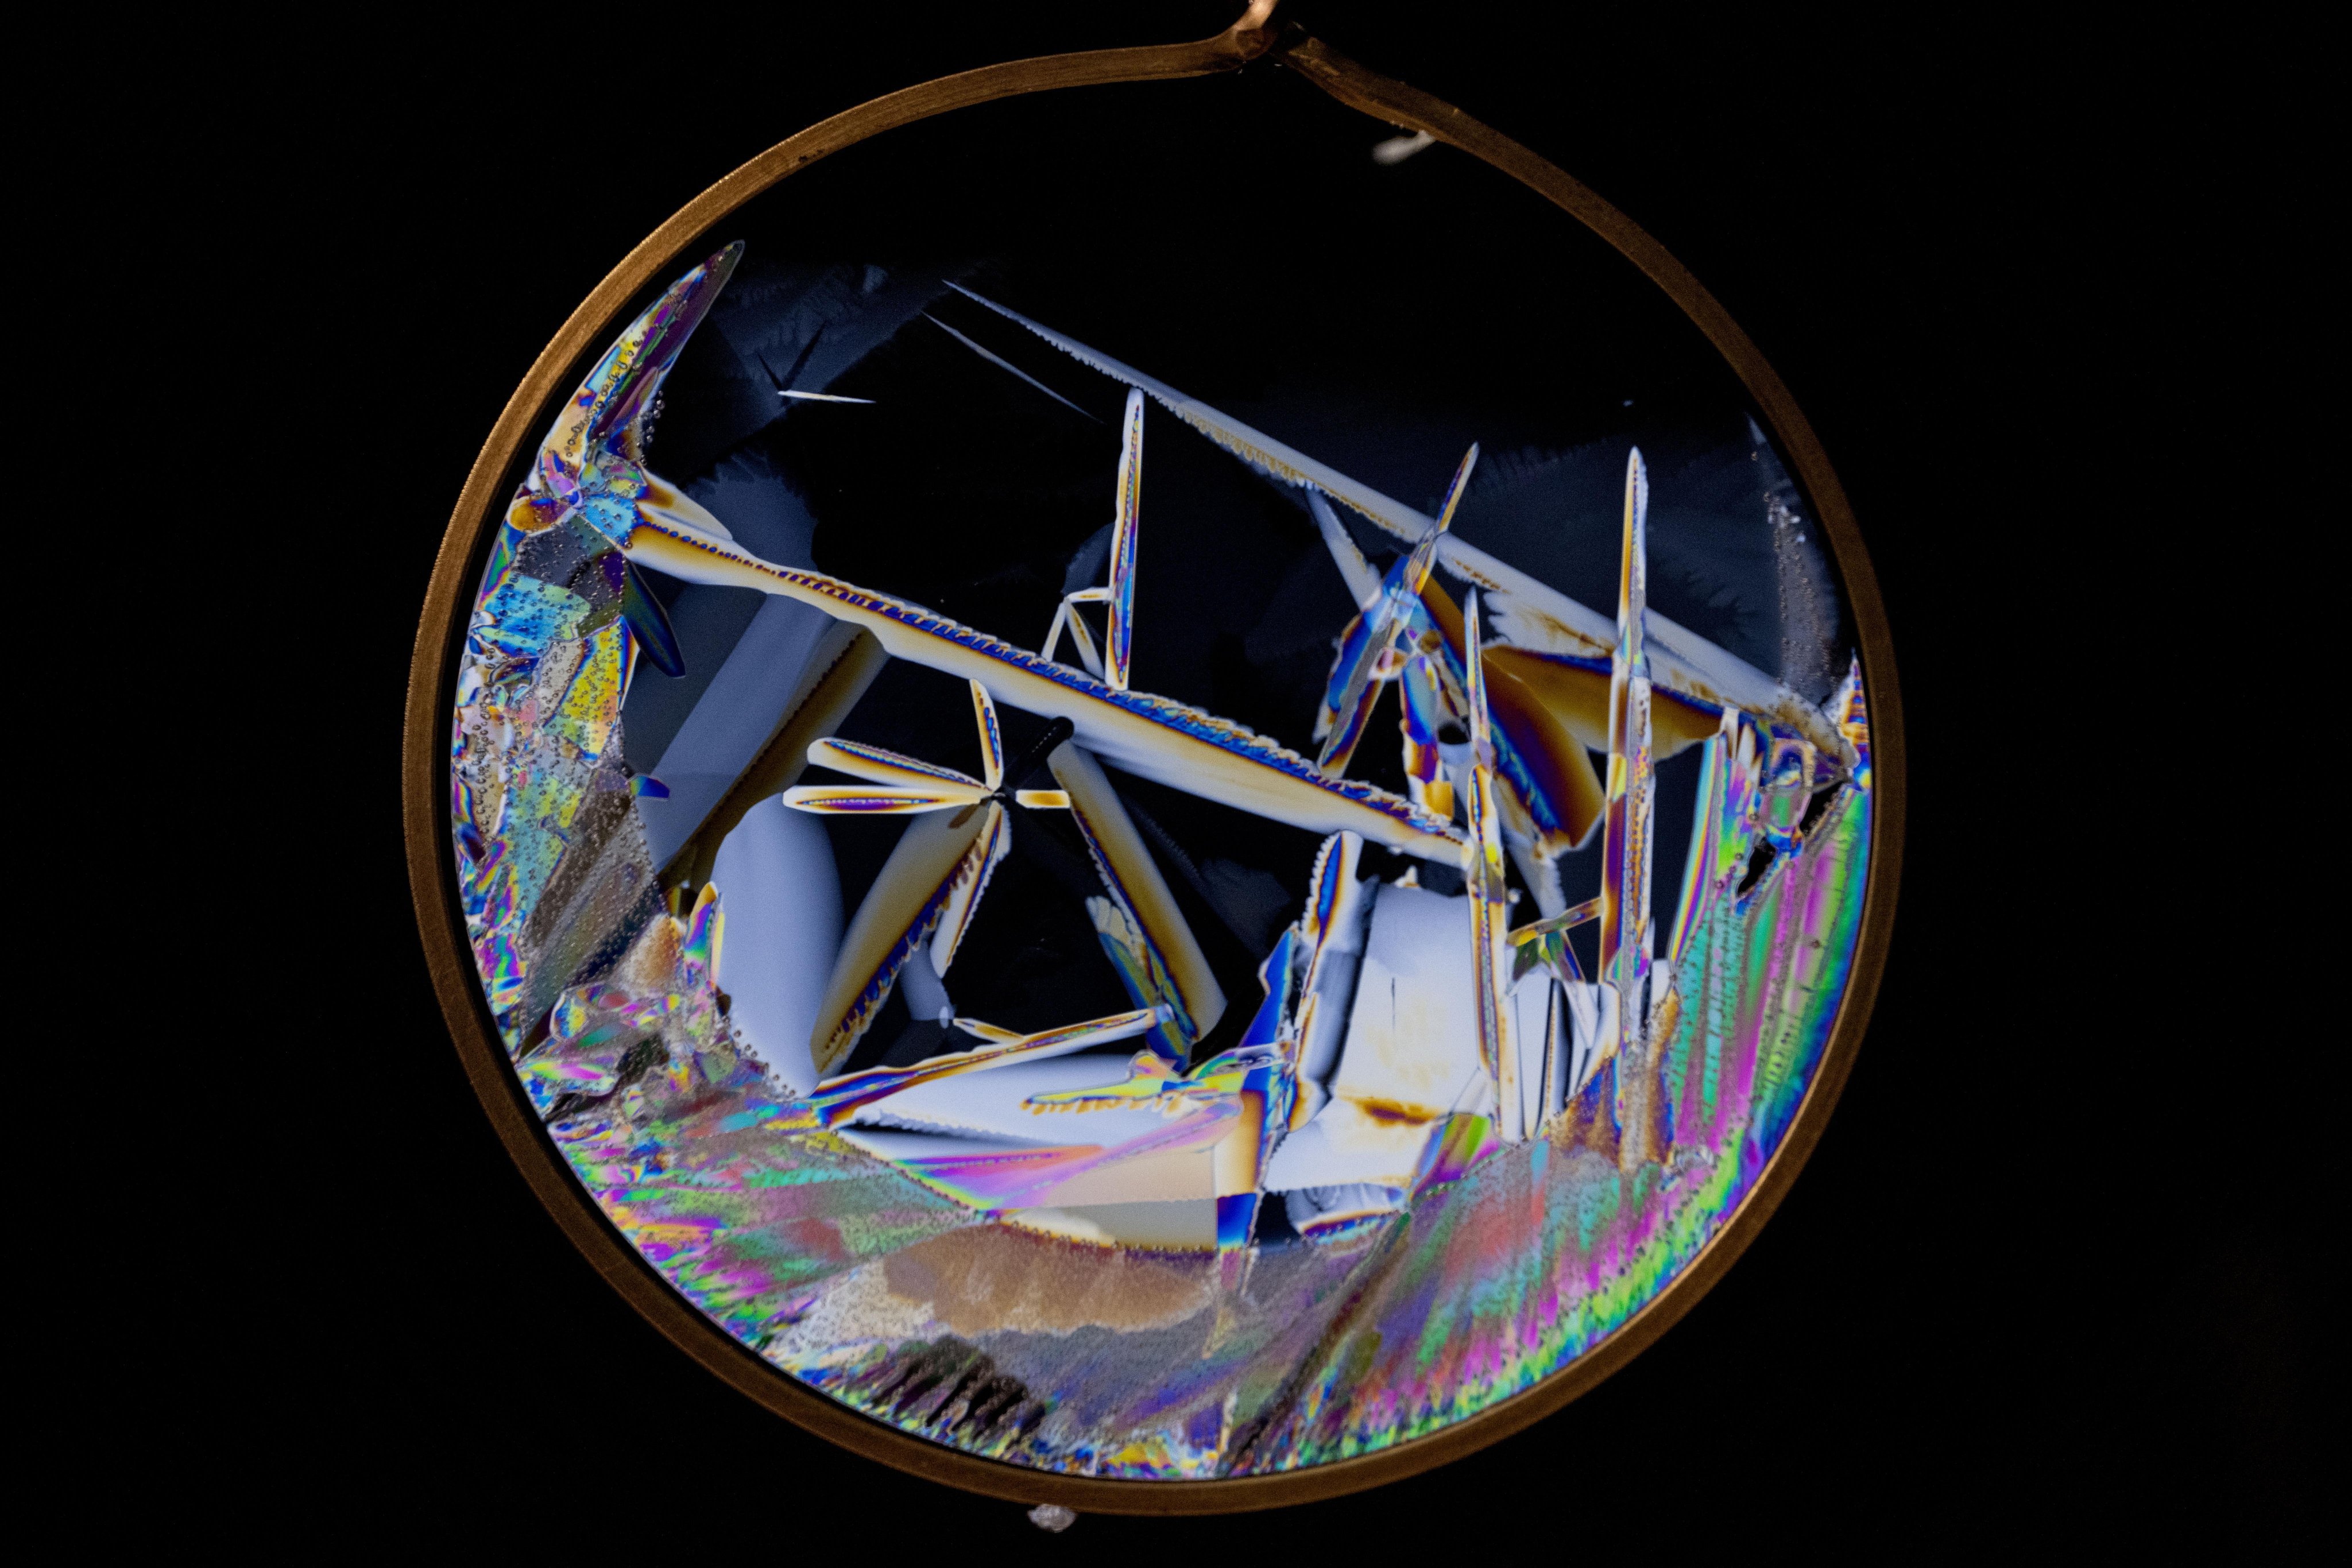
\includegraphics[width=0.5\textwidth]{lens.jpeg}
    \caption{Idk what this is.}
    \label{lens_figure}
\end{figure}

Figure \ref{lens_figure} is pretty for the following reasons:
\begin{itemize}
    \item nice colors
    \item interesting shapes
\end{itemize}

Here are some equations:
\begin{enumerate}
    \item $e^{i \pi} = -1$
\end{enumerate}

Here is some dislay math:
\[
1 + 1 = 2
\]

\section{Table}
Here is a table \ref{table:table}:

\begin{table}[h!]
\centering
\begin{tabular}{|c|c|c|}
    \hline
    0 & 1 & 2 \\
    \hline
    0 & 1 & 2 \\
    \hline
\end{tabular}
\caption{Table caption}
\label{table:table}
\end{table}


\end{document}

